% !TEX program = xelatex
\documentclass[11pt,a4paper,twoside]{report}

\usepackage[table]{xcolor}
\usepackage[a4paper,margin=28mm]{geometry}
\usepackage{graphicx}
\usepackage{microtype}
\usepackage{setspace}
\usepackage{parskip}
\usepackage{booktabs}
\usepackage{tabularx}
\usepackage{longtable}
\usepackage{array}
\usepackage{multirow}
\usepackage{enumitem}
\usepackage{amssymb}
\usepackage{pifont}
\usepackage{fontawesome5}
\usepackage{listings}
\usepackage[hyphens]{url}
\usepackage{tcolorbox}
\usepackage{tikz}
\usetikzlibrary{arrows.meta,positioning,shapes.geometric,fit,calc,chains,backgrounds}

\usepackage[hidelinks]{hyperref}
\usepackage{fontspec}
\usepackage[capitalize,noabbrev]{cleveref}

\definecolor{sapblue}{HTML}{0B5FA5}
\definecolor{sapgreen}{HTML}{00695C}
\definecolor{sapamber}{HTML}{B8360F}
\definecolor{sapgrey}{HTML}{546E7A}
\definecolor{regred}{HTML}{B71C1C}
\definecolor{regblue}{HTML}{1565C0}
\definecolor{reggreen}{HTML}{2E7D32}
\definecolor{reggrey}{HTML}{546E7A}
\definecolor{regamber}{HTML}{F0AB00}
\definecolor{pathcolor}{HTML}{004D40}
\definecolor{sapmidnight}{HTML}{1C2B39}

\lstdefinelanguage{jsonx}{
basicstyle=\ttfamily\small,
columns=fullflexible,
breaklines=true,
showstringspaces=false,
comment=[l]{//},
morestring=[b]",
stringstyle=\color{sapgreen},
keywordstyle=\color{sapblue},
}

\lstdefinelanguage{yamlx}{
keywords={true,false,null,y,n},
keywordstyle=\color{sapblue}\bfseries,
basicstyle=\ttfamily\small,
sensitive=false,
comment=[l]{\#},
morecomment=[s]{/*}{*/},
commentstyle=\color{sapgreen}\ttfamily,
stringstyle=\color{sapamber}\ttfamily,
moredelim=[l][\color{sapmidnight}]{\:},
morestring=[b]',
morestring=[b]",
}

\newtcolorbox{adrbox}[2][]{colback=blue!5,colframe=blue!75!black,fonttitle=\bfseries,title=ADR: #2,#1}
\newcommand{\filepath}[1]{{\color{pathcolor}\path{#1}}}
\newcommand{\artifact}[1]{\texttt{\textcolor{sapblue}{#1}}}
\newcommand{\reqid}[1]{\texttt{\textcolor{regred}{#1}}}
\newcolumntype{L}[1]{>{\raggedright\arraybackslash}p{#1}}

\raggedbottom
\onehalfspacing
\setlist{topsep=2pt,itemsep=1pt,parsep=0pt}
\setlength{\emergencystretch}{3em}
\tolerance=1000
\hbadness=10000

\begin{document}

\title{\vspace{-2em}\Large .clinerules Agent Swarm \\
\textbf{Specification and Delivery Model} \\
\large Cross-Domain Supplement for SAP OSS \\
\small Ref: \texttt{CLN-SWARM-2026-v1.1.1}}
\author{SAP-OSS Platform Engineering}
\date{April 2026 (Revised)}

\maketitle

\chapter{Frontmatter}
\label{ch:frontmatter}

\tableofcontents
\clearpage

\section{Purpose}

This supplementary specification defines how \artifact{.clinerules}
files are used as agent contracts across the SAP OSS repository. It is
not a replacement for the four domain specifications. Instead, it is
the operational layer that turns those specifications into a governed
agent fleet: development agents, runtime-monitor agents, and the swarm
that delivers the artefacts under \filepath{docs/pdf/specs/}.

\section{Normative relationship to the regulations specification}

This document is subordinate to
\filepath{docs/pdf/specs/regulations-spec.pdf}. The regulations book
defines the governing obligations for agentic AI; this document
translates those obligations into repository-level rule-pack patterns,
path conventions, validation harnesses, and swarm responsibilities.

\section{Scope}

The specification covers:
\begin{itemize}
\item development-time \artifact{.clinerules} files for domain
implementation and maintenance agents;
\item runtime-monitor \artifact{.clinerules} companions that watch
live agent behaviour and evidence;
\item path conventions for placing these rule files in the codebase;
\item the minimum contract each rule pack must encode;
\item the swarm model used to deliver and maintain
\filepath{docs/pdf/specs/}.
\end{itemize}

Out of scope:
\begin{itemize}
\item inventing new governance obligations that contradict the
regulations specification;
\item replacing the domain specifications with agent rules;
\item defining a specific external agent runtime implementation.
\end{itemize}

\section{Deliverables required by this specification}

\begin{table}[htbp]
\centering
\footnotesize
\caption{Primary deliverables.}
\label{tab:deliverables}
\begin{tabularx}{\textwidth}{@{}l l X@{}}
\toprule
\textbf{Deliverable} & \textbf{Path pattern} & \textbf{Purpose} \\
\midrule
Development agent rule pack & \filepath{src/<domain>/.clinerules} & Implementation, migration, maintenance, and test expectations for a domain or service. \\
Runtime monitor rule pack & \filepath{src/<domain>/.clinerules.runtime-monitor} & Live monitoring, alerting, evidence correlation, and fail-closed rules. \\
Supplementary agent spec & \filepath{docs/latex/specs/clinerules-agents/} & Cross-domain operating model for rule packs and swarm delivery. \\
Validation harness & colocated tests & Structural and benchmark validation of rule packs. \\
\bottomrule
\end{tabularx}
\end{table}

\section{Current repository examples}

The repository already contains rule-pack precedents:
\begin{itemize}
\item \filepath{.clinerules}
\item \filepath{src/generativeUI/.clinerules}
\item \filepath{src/training/.clinerules}
\item \filepath{src/training/.clinerules.runtime-monitor}
\end{itemize}

This specification extends that pattern by requiring the regulations
domain to own its own development and runtime-monitor rule packs under
\filepath{src/intelligence/}.
\chapter{Overview}
\label{ch:overview}

\section{What a .clinerules agent is}

A \artifact{.clinerules} file is a local contract for an agent. It is
not application code and not a product requirement document. It is the
bridge between the two:
\begin{itemize}
\item the specification states what must be true;
\item the \artifact{.clinerules} file states how an agent must work
in this repository to keep that true.
\end{itemize}

\section{Two mandatory agent types}

Every governed domain should have two mandatory agent contracts.

\subsection*{1. Development agent}

The development agent owns implementation, integration, migration, test
obligations, and completion criteria. Its contract lives in
\filepath{src/<domain>/.clinerules}.

\subsection*{2. Runtime-monitor agent}

The runtime-monitor agent owns health criteria, alert conditions,
evidence correlation, and escalation behaviour. Its contract lives in
\filepath{src/<domain>/.clinerules.runtime-monitor}.

\section{Why the split is required}

\begin{adrbox}{Separation of construction from supervision}
A single rule file is not enough for a governed agentic platform. The
development agent must optimize for implementation correctness and
contract coherence. The runtime-monitor agent must optimize for
observability, alerting precision, and fail-closed behaviour. Keeping
them separate avoids blending build-time convenience with runtime risk
control.
\end{adrbox}

\section{Why a swarm is needed}

The artefacts in \filepath{docs/pdf/specs/} are cross-domain. They span
Arabic, TB, regulations, Simula, shared fragments, and the
implementation rule packs that keep those books honest. A single agent
can draft changes, but a reliable delivery model needs multiple roles:
\begin{itemize}
\item domain specialists who know their code and contracts;
\item regulatory specialists who impose the governance envelope;
\item runtime monitors that validate live control assumptions;
\item documentation and PDF build specialists who assemble and
validate the published specifications.
\end{itemize}

\section{Rule-pack lifecycle states}
\label{sec:lifecycle-states}

A rule-pack transitions through defined lifecycle states to ensure
governance integrity before enforcement begins.

\begin{table}[htbp]
\centering
\footnotesize
\caption{Rule-pack lifecycle states.}
\label{tab:lifecycle-states}
\begin{tabularx}{\textwidth}{@{}l l X@{}}
\toprule
\textbf{State} & \textbf{Trigger} & \textbf{Behaviour} \\
\midrule
\texttt{DRAFT} & Feature branch with \texttt{status: draft} frontmatter & Structural validity MAY be checked; CI/CD gates SHALL NOT block on draft packs. \\
\texttt{REVIEW} & Pull request opened against default branch & Full validation harness runs; reviewers must approve before merge. \\
\texttt{ACTIVE} & Merged to default branch & Pack is enforced; all agents must comply with its obligations. \\
\texttt{DEPRECATED} & \texttt{status: deprecated} frontmatter added & Pack remains enforced for one release cycle; agents receive deprecation warnings. \\
\texttt{RETIRED} & Removed from repository & Pack is no longer enforced; historical references remain in audit logs. \\
\bottomrule
\end{tabularx}
\end{table}

\subsection{Lifecycle invariants}

\begin{itemize}
\item A rule-pack SHALL be considered \textbf{active} only when merged
to the default branch without a \texttt{status: draft} or
\texttt{status: deprecated} frontmatter field.
\item During development, a rule-pack MAY reside in a feature branch
and be marked as \texttt{DRAFT} via frontmatter. Draft packs SHALL
NOT block CI/CD gates, but their structural validity MAY be checked.
\item Deprecation requires a minimum one-release window before
retirement to allow dependent agents to adapt.
\item Retirement does not erase audit history; all actions taken under
the pack remain attributable.
\end{itemize}
\chapter{Regulatory Alignment}
\label{ch:reg-alignment}

\section{Principle}

Every \artifact{.clinerules} pack in this repository must inherit the
governance obligations defined by
\filepath{docs/pdf/specs/regulations-spec.pdf}. Alignment is not
optional for domain packs. It is the precondition for claiming that an
agent is suitable for development, deployment, or runtime supervision.

\section{Minimum mapping from regulations to rule packs}

\begin{table}[htbp]
\centering
\footnotesize
\caption{Required mapping from regulations obligations to rule-pack behaviour.}
\label{tab:reg-map}
\begin{tabularx}{\textwidth}{@{}L{3.2cm}L{3.0cm}X@{}}
\toprule
\textbf{Regulations requirement} & \textbf{Source in regulations spec} & \textbf{Rule-pack implication} \\
\midrule
\reqid{REG-MGF-2.1.2-001} explicit tool allow-list, deny-by-default & Chapter 3, Pillar 1 & Development agents must cite the allow-list source; runtime agents must alert on undeclared tool use or path bypass. \\
\reqid{REG-MGF-2.1.2-002} per-action identity attribution & Chapter 3, Pillar 1 and Chapter 10 & Development agents must require identity envelope propagation and audit-event schema alignment; runtime agents must fail closed on missing identity evidence. \\
\reqid{REG-MGF-2.1.2-003} impact-limiting boundaries & Chapter 3, Pillar 1 & Development agents must preserve read-only defaults, environment segregation, and explicit escalation for higher-risk actions. \\
\reqid{REG-MGF-2.2.1-001} named lifecycle responsibilities & Chapter 3, Pillar 2 & Every rule pack must name its owning domain and the responsibilities of the agent. \\
\reqid{REG-MGF-2.2.2-001} human approval checkpoints & Chapter 3, Pillar 2 & Runtime agents must know when to escalate, block, or require human acknowledgement. \\
\reqid{REG-MGF-2.3.1-001} technical controls on planning, tools, protocols & Chapter 3, Pillar 3 & Development packs must encode source of truth, read-first files, non-negotiable engineering rules, and completion blockers. \\
\reqid{REG-MGF-2.3.2-001} pre-deployment evaluation & Chapter 3, Pillar 3 and Chapter 6 & Development packs must define runnable validation steps and conformance expectations. \\
\reqid{REG-MGF-2.3.3-001} staged rollout and rollback & Chapter 3, Pillar 3 and Chapter 8 & Runtime packs must recognize degradation ladders, rollback triggers, and canary-style alerting. \\
\reqid{REG-MGF-2.3.3-002} continuous monitoring & Chapter 3, Pillar 3 and Chapter 8 & Runtime packs must define metrics, thresholds, severities, response rules, and circuit-break conditions. \\
\bottomrule
\end{tabularx}
\end{table}

\section{Identity and audit obligations}

Rule packs that touch live execution must align to the identity and
audit schemas under \filepath{docs/schema/regulations/}:
\begin{itemize}
\item \filepath{agent-identity.schema.json}
\item \filepath{request-identity.schema.json}
\item \filepath{audit-event.schema.json}
\end{itemize}

This means:
\begin{itemize}
\item no agent action without a request identity;
\item no action without an attributable agent identity;
\item no irreversible side effect unless the audit path is in a
valid pre-action state;
\item no runtime monitor may declare a run healthy if the evidence
chain is partial.
\end{itemize}

\section{Monitoring obligations}

Runtime-monitor packs must inherit the monitoring model from Chapter 8
of the regulations book:
\begin{itemize}
\item explicit metrics;
\item explicit detection triggers;
\item explicit severity levels;
\item explicit routing and escalation;
\item explicit graceful degradation and circuit-break behaviour.
\end{itemize}

The minimum thresholds that runtime packs must encode include:
\begin{itemize}
\item schema-violation surge above 5\% of requests;
\item refusal rate above 3x baseline;
\item topic similarity below 0.7;
\item latency p95 above 1.5x baseline;
\item circuit-break escalation after 3 consecutive critical alerts in
15 minutes.
\end{itemize}

\section{Baseline warm-up period}
\label{sec:baseline-warmup}

For newly deployed agents or after major model/rule-pack changes, the
runtime-monitor SHOULD enter a \texttt{LEARNING} state for a defined
period before enforcing baseline-dependent thresholds. This prevents
false-positive alert storms during cold-start conditions.

\subsection{Warm-up parameters}

\begin{table}[htbp]
\centering
\footnotesize
\caption{Baseline warm-up configuration.}
\label{tab:warmup-config}
\begin{tabularx}{\textwidth}{@{}l l X@{}}
\toprule
\textbf{Parameter} & \textbf{Default} & \textbf{Description} \\
\midrule
\texttt{warmup\_duration} & 24 hours & Minimum time before transitioning to \texttt{ENFORCING}. \\
\texttt{warmup\_requests} & 1{,}000 & Minimum request count before transitioning. \\
\texttt{warmup\_trigger} & Both & Transition occurs when \emph{both} duration and request count are satisfied. \\
\bottomrule
\end{tabularx}
\end{table}

\subsection{Behaviour during warm-up}

During the \texttt{LEARNING} state:
\begin{itemize}
\item Alerts SHALL be logged to the audit trail but SHALL NOT be
routed to on-call escalation channels.
\item The system MUST automatically establish rolling baselines
(P50/P95) for latency, refusal rate, and topic distribution.
\item Absolute thresholds (e.g., schema-violation surge above 5\%)
remain enforced; only baseline-relative thresholds (e.g., 3x
baseline) are suspended.
\item The warm-up state MUST be visible in the monitoring dashboard
with a countdown indicator.
\end{itemize}

\subsection{Transition to enforcing state}

After the warm-up period completes:
\begin{itemize}
\item The monitor transitions to \texttt{ENFORCING} state
automatically.
\item An informational alert is logged recording the established
baselines (P50, P95, mean for each metric).
\item All baseline-relative thresholds become active.
\item Manual override to extend warm-up requires explicit operator
approval with audit justification.
\end{itemize}

\subsection{Warm-up reset triggers}

The warm-up period MUST reset when any of the following occur:
\begin{itemize}
\item Major model version change (detected via
\filepath{src/intelligence/model-registry.yaml});
\item Rule-pack version increment in the governing
\filepath{.clinerules} file;
\item Explicit operator command with audit justification;
\item Infrastructure migration affecting the monitored endpoint.
\end{itemize}
\chapter{Agent Rule-Pack Architecture}
\label{ch:architecture}

\section{Repository path convention}

\begin{table}[htbp]
\centering
\footnotesize
\caption{Standard path convention for .clinerules packs.}
\label{tab:path-convention}
\begin{tabularx}{\textwidth}{@{}l X@{}}
\toprule
\textbf{Path} & \textbf{Meaning} \\
\midrule
\filepath{.clinerules} & Repository-wide or umbrella rules that are not owned by a single implementation subtree. \\
\filepath{src/<domain>/.clinerules} & Development and maintenance contract for one domain or service family. \\
\filepath{src/<domain>/.clinerules.runtime-monitor} & Runtime monitoring and alerting contract for the same domain or service family. \\
\filepath{src/<domain>/tests/test_clinerules_contracts.py} or equivalent & Validation harness that proves the rule packs are structurally complete and benchmarked. \\
\bottomrule
\end{tabularx}
\end{table}

\section{Frontmatter format definition}
\label{sec:frontmatter-format}

Every \artifact{.clinerules} pack MUST begin with a YAML frontmatter
block delimited by triple-dashes (\texttt{---}). This block defines
the mission, state, and governance linkage for the agent.

\begin{adrbox}{YAML-between-Dashes}
We mandate YAML frontmatter to ensure that metadata (version, domain,
conformance tags) is machine-readable by the validation harness without
requiring a full markdown parser.
\end{adrbox}

\section{Minimum contents of a development pack}

Every development rule pack must encode, at minimum:
\begin{enumerate}
\item purpose and mission;
\item source of truth;
\item read-first files;
\item current repo reality and known issue registry;
\item definition of done;
\item non-negotiable engineering rules;
\item contract rules for schemas, payloads, and artefacts;
\item integration rules for adjacent systems;
\item pre-change checklist;
\item post-change smoke tests;
\item completion blockers.
\end{enumerate}

\section{Minimum contents of a runtime-monitor pack}

Every runtime-monitor pack must encode, at minimum:
\begin{enumerate}
\item purpose and mission;
\item source of truth;
\item evidence sources;
\item healthy versus unhealthy criteria;
\item critical, high, medium, and informational conditions;
\item condition codes;
\item response rules and escalation path;
\item operator triage checklist;
\item minimum evidence required to close an alert.
\end{enumerate}

\section{Cross-domain inventory required by this specification}

\begin{table}[htbp]
\centering
\footnotesize
\caption{Target rule-pack inventory.}
\label{tab:inventory}
\begin{tabularx}{\textwidth}{@{}l l X@{}}
\toprule
\textbf{Area} & \textbf{Path} & \textbf{Role} \\
\midrule
Shared repository & \filepath{.clinerules} & Repo-wide documentation and standards baseline. \\
Generative UI & \filepath{src/generativeUI/.clinerules} & Deployment and monitoring standards for the UI stack. \\
Simula training & \filepath{src/training/.clinerules} & Implementation and migration contract for the Simula path. \\
Simula runtime & \filepath{src/training/.clinerules.runtime-monitor} & Monitoring and alerting contract for Simula runs. \\
Regulations development & \filepath{src/intelligence/.clinerules} & Governance-runtime implementation contract. \\
Regulations runtime & \filepath{src/intelligence/.clinerules.runtime-monitor} & Monitoring, alerting, and fail-closed contract for governance runtime. \\
\bottomrule
\end{tabularx}
\end{table}

\section{Rule-pack inheritance conflict detection}
\label{sec:conflict-detection}

The validation harness MUST include automated checks that ensure
domain-specific packs do not override critical regulatory constraints
with less restrictive values. This is the technical enforcement of the
``inherit, never weaken'' principle.

\subsection{Inheritance hierarchy}

Rule packs inherit in the following order (most general to most
specific):
\begin{enumerate}
\item \textbf{Repository-level}: \filepath{.clinerules} (baseline)
\item \textbf{Intelligence-level}: \filepath{src/intelligence/.clinerules}
(regulations envelope)
\item \textbf{Domain-level}: \filepath{src/<domain>/.clinerules}
(domain-specific constraints)
\end{enumerate}

\subsection{Critical safety flags}

The following flags are designated as \textbf{safety-critical} and
may only be \emph{tightened} (made more restrictive) by child packs,
never \emph{loosened}:

\begin{table}[htbp]
\centering
\footnotesize
\caption{Safety-critical flags and their tightening direction.}
\label{tab:safety-flags}
\begin{tabularx}{\textwidth}{@{}l l X@{}}
\toprule
\textbf{Flag} & \textbf{Tightening direction} & \textbf{Violation example} \\
\midrule
\texttt{deny\_by\_default} & \texttt{false} $\rightarrow$ \texttt{true} only & Domain sets \texttt{true} $\rightarrow$ \texttt{false}. \\
\texttt{allow\_unlisted\_tools} & \texttt{true} $\rightarrow$ \texttt{false} only & Domain enables unlisted tools when parent denies. \\
\texttt{require\_identity\_envelope} & \texttt{false} $\rightarrow$ \texttt{true} only & Domain disables identity requirement. \\
\texttt{audit\_before\_action} & \texttt{false} $\rightarrow$ \texttt{true} only & Domain disables pre-action audit. \\
\texttt{circuit\_break\_enabled} & \texttt{false} $\rightarrow$ \texttt{true} only & Domain disables circuit breaker. \\
\texttt{max\_retries} & May only \emph{decrease} & Domain increases retry limit beyond parent. \\
\texttt{timeout\_ms} & May only \emph{decrease} & Domain increases timeout beyond parent. \\
\bottomrule
\end{tabularx}
\end{table}

\subsection{Automated conflict detection}

The validation harness SHALL:
\begin{enumerate}
\item Load packs in inheritance order (Repository $\rightarrow$
Intelligence $\rightarrow$ Domain).
\item For each safety-critical flag, compare the child value against
the parent value.
\item If a child value is less restrictive than the parent, emit a
\textbf{CONFLICT\_ERROR} with:
\begin{itemize}
\item the flag name;
\item the parent path and value;
\item the child path and attempted value;
\item the allowed tightening direction.
\end{itemize}
\item Block CI/CD pipeline progression if any conflict is detected.
\end{enumerate}

\subsection{Conflict resolution workflow}

When a conflict is detected:
\begin{enumerate}
\item The domain team MUST either:
\begin{itemize}
\item remove the conflicting override;
\item or request a formal exception via the Controls Architecture
Team.
\end{itemize}
\item Exceptions require documented risk acceptance and a time-bound
remediation plan.
\item All exceptions MUST be logged to
\filepath{docs/schema/common/exceptions-registry.yaml} (validated
against \filepath{exceptions-registry.schema.json}) with:
\begin{itemize}
\item exception ID;
\item requesting domain;
\item justification;
\item expiry date;
\item approving authority.
\end{itemize}
\end{enumerate}
\chapter{Regulatory Agents}
\label{ch:reg-agents}

\section{Why the regulations agents live in \texttt{src/intelligence}}

The repository does not contain a standalone
\filepath{src/regulations/} service. The concrete runtime surface for
regulations obligations lives in and around:
\begin{itemize}
\item \filepath{src/intelligence/ai-core-pal/}
\item \filepath{src/intelligence/monitoring/}
\item \filepath{src/intelligence/analytics/}
\end{itemize}

The regulations development and runtime-monitor rule packs therefore
belong under \filepath{src/intelligence/}.

\section{Required regulatory development agent}

The development pack at \filepath{src/intelligence/.clinerules} must
govern any work that claims to implement the regulations domain. It
must be schema-backed by:
\begin{itemize}
\item \filepath{docs/schema/regulations/requirement.schema.json}
\item \filepath{docs/schema/regulations/conformance-tool.schema.json}
\item \filepath{docs/schema/regulations/agent-identity.schema.json}
\item \filepath{docs/schema/regulations/request-identity.schema.json}
\item \filepath{docs/schema/regulations/audit-event.schema.json}
\item \filepath{docs/schema/regulations/capability-monitoring-metrics.schema.json}
\end{itemize}

It must point agents to the live implementation surface, including:
\begin{itemize}
\item \filepath{src/intelligence/ai-core-pal/mcp_server/btp_pal_mcp_server.py}
\item \filepath{src/intelligence/ai-core-pal/data_products/registry.yaml}
\item \filepath{src/intelligence/analytics/anomaly_detector.py}
\item \filepath{src/intelligence/monitoring/kill_switch_monitor.py}
\item \filepath{src/intelligence/ai-core-pal/tests/test_mcp_server.py}
\end{itemize}

\section{Required regulatory runtime-monitor agent}

The runtime-monitor pack at
\filepath{src/intelligence/.clinerules.runtime-monitor} must supervise:
\begin{itemize}
\item allow-list bypass and undeclared tool use;
\item missing or partial identity envelopes;
\item audit reservation failures and orphaned completions;
\item monitoring metric gaps;
\item schema-violation surges;
\item refusal-rate spikes, latency spikes, topic drift, and related
degradation triggers;
\item circuit-break conditions and alert routing.
\end{itemize}

\section{Minimum acceptance criteria for the regulations agent pair}

\begin{enumerate}
\item The development pack cites the regulations specification and
schema files as source of truth.
\item The runtime-monitor pack cites the monitoring and identity
chapters as source of truth.
\item Both packs name concrete code paths and test entry points that
exist in the repository.
\item A validation harness checks both packs for structural
completeness and benchmark quality.
\item The combined pair benchmarks at least as strongly as the
existing \filepath{src/generativeUI/.clinerules} baseline on
operational specificity.
\end{enumerate}

\section{Ingress overlay requirements}
\label{sec:ingress-overlay}

The primary regulatory pair lives under \filepath{src/intelligence/},
because that is where the core governance runtime lives. However, if a
service in \filepath{src/generativeUI/gateway/} is the primary entry
point for external traffic \textbf{AND} it handles
authentication/authorization token extraction, then a companion pack at
\filepath{src/generativeUI/gateway/.clinerules.runtime-monitor} is
\textbf{MANDATORY}, not merely recommended. This mandatory pack SHOULD be
automatically generated from the primary intelligence pack plus a
gateway-specific overlay template to minimize maintenance overhead.

\subsection{Mandatory ingress enforcement}

When the gateway is the external traffic entry point, the ingress
overlay MUST enforce:

\begin{enumerate}
\item \textbf{Header propagation validation}: The monitor MUST verify
that required headers (\texttt{X-Request-ID}, \texttt{X-Agent-Identity},
\texttt{X-Correlation-ID}) are present and correctly formatted before
requests reach internal services.
\item \textbf{Early rejection of invalid requests}: Requests missing
required identity claims MUST be rejected at the gateway level with
appropriate HTTP status codes (401/403) and audit logging.
\item \textbf{Identity envelope integrity}: The gateway MUST validate
that identity tokens have not been tampered with and originate from
trusted issuers.
\item \textbf{Rate limiting enforcement}: Per-identity rate limits
MUST be enforced at the gateway to prevent resource exhaustion attacks.
\end{enumerate}

\subsection{Ingress overlay minimum contents}

The ingress runtime-monitor pack at
\filepath{src/generativeUI/gateway/.clinerules.runtime-monitor} MUST
include:

\begin{table}[htbp]
\centering
\footnotesize
\caption{Ingress overlay minimum requirements.}
\label{tab:ingress-requirements}
\begin{tabularx}{\textwidth}{@{}l X@{}}
\toprule
\textbf{Section} & \textbf{Required content} \\
\midrule
Evidence sources & Gateway access logs, authentication service logs, rate-limiter metrics. \\
Critical conditions & Missing identity headers, invalid tokens, rate limit exceeded, upstream timeout. \\
Alert routing & Security team for identity violations; platform team for availability issues. \\
Circuit-break triggers & 3+ consecutive authentication failures from same source in 1 minute. \\
\bottomrule
\end{tabularx}
\end{table}

\subsection{Inheritance from primary regulatory pair}

The ingress overlay MUST inherit from (not replace) the primary
regulatory runtime-monitor at
\filepath{src/intelligence/.clinerules.runtime-monitor}. Specifically:
\begin{itemize}
\item All safety-critical flags from the parent MUST be preserved or
tightened (see \cref{sec:conflict-detection}).
\item The ingress overlay MAY add gateway-specific conditions but
MUST NOT remove or weaken inherited conditions.
\item Audit events from the gateway MUST conform to the same
\filepath{docs/schema/regulations/audit-event.schema.json} as the
core governance runtime.
\end{itemize}

\subsection{Exception for non-external gateways}

If the gateway at \filepath{src/generativeUI/gateway/} handles
\emph{only} internal service-to-service traffic (not external user
requests), the ingress overlay MAY be designated as \texttt{OPTIONAL}
with documented justification in the rule pack frontmatter:
\begin{verbatim}
# Ingress overlay: OPTIONAL
# Justification: Gateway handles internal traffic only.
# External entry point: src/external-gateway/
# Reviewed by: [Approver ID]
# Review date: [Date]
\end{verbatim}
\chapter{Spec-Drift Audit Agent}
\label{ch:spec-drift-agent}

\section{Purpose and scope}

The Spec-Drift Audit Agent is a specialized governance agent that monitors
synchronization between three artifact types:

\begin{enumerate}
\item \textbf{LaTeX specifications} in \filepath{docs/latex/specs/}
\item \textbf{JSON/YAML schemas} in \filepath{docs/schema/}
\item \textbf{Implementation code} in \filepath{src/}
\end{enumerate}

When any of these artifacts change, the agent ensures related artifacts are
also updated to maintain consistency. This prevents \emph{specification drift}
where documentation diverges from implementation.

\section{Agent configuration files}

\subsection{Primary configuration}

\begin{table}[htbp]
\centering
\footnotesize
\caption{Spec-drift agent configuration files.}
\label{tab:spec-drift-files}
\begin{tabularx}{\textwidth}{@{}l X@{}}
\toprule
\textbf{File} & \textbf{Purpose} \\
\midrule
\filepath{.clinerules.spec-drift-auditor} & Agent behavior rules and drift type definitions \\
\filepath{docs/schema/spec-code-mapping.yaml} & Traceability registry mapping artifacts \\
\filepath{docs/schema/drift-exceptions.yaml} & Approved exceptions with expiration \\
\filepath{scripts/spec-drift/audit.py} & Drift detection engine implementation \\
\filepath{scripts/spec-drift/pre-commit-hook.sh} & Git pre-commit hook \\
\filepath{.github/workflows/spec-drift-audit.yml} & CI/CD workflow \\
\bottomrule
\end{tabularx}
\end{table}

\subsection{Domain-specific rule packs}

Each specification directory contains a \filepath{.clinerules} file that
defines domain-specific synchronization rules:

\begin{table}[htbp]
\centering
\footnotesize
\caption{Domain-specific .clinerules locations.}
\label{tab:domain-clinerules}
\begin{tabularx}{\textwidth}{@{}l X@{}}
\toprule
\textbf{Location} & \textbf{Domain} \\
\midrule
\filepath{docs/schema/.clinerules} & Schema governance and data contracts \\
\filepath{docs/latex/specs/.clinerules} & Specification directory standards \\
\filepath{docs/latex/specs/simula/.clinerules} & Training data framework \\
\filepath{docs/latex/specs/regulations/.clinerules} & AI regulatory compliance \\
\filepath{docs/latex/specs/arabic/.clinerules} & Arabic AP Invoice processing \\
\filepath{docs/latex/specs/tb/.clinerules} & Trial Balance review \\
\filepath{docs/latex/specs/tb-hitl/.clinerules} & TB business requirements \\
\filepath{docs/latex/specs/arabic-hitl/.clinerules} & Arabic business requirements \\
\filepath{docs/latex/specs/clinerules-agents/.clinerules} & This specification \\
\bottomrule
\end{tabularx}
\end{table}

\section{Drift types detected}
\label{sec:drift-types}

The audit agent detects eight categories of specification drift:

\begin{table}[htbp]
\centering
\footnotesize
\caption{Drift type classification.}
\label{tab:drift-types}
\begin{tabularx}{\textwidth}{@{}l l X@{}}
\toprule
\textbf{Code} & \textbf{Severity} & \textbf{Description} \\
\midrule
DRIFT-001 & HIGH/MEDIUM & Schema-Spec Drift: Schema field changed without spec update \\
DRIFT-002 & CRITICAL/HIGH & Code-Schema Drift: Code references non-existent schema fields \\
DRIFT-003 & CRITICAL/HIGH & Code-Spec Drift: Code behavior contradicts spec requirement \\
DRIFT-004 & HIGH/MEDIUM & Version Drift: Version numbers out of sync \\
DRIFT-005 & CRITICAL/HIGH & Cross-Domain Drift: Shared enum changed without updating consumers \\
DRIFT-006 & HIGH/MEDIUM & Threshold Drift: Code uses different threshold than spec \\
DRIFT-007 & CRITICAL/HIGH & State Machine Drift: Workflow states differ between code and spec \\
DRIFT-008 & CRITICAL/HIGH & API Contract Drift: API differs from spec documentation \\
\bottomrule
\end{tabularx}
\end{table}

\section{Enforcement mechanisms}
\label{sec:enforcement}

\textbf{CRITICAL: To guarantee spec-drift checks always run, multiple
enforcement layers are required.} No single mechanism is sufficient.

\subsection{Layer 1: CI/CD enforcement (Mandatory)}

The GitHub Actions workflow at \filepath{.github/workflows/spec-drift-audit.yml}
provides server-side enforcement that \textbf{cannot be bypassed} by developers:

\begin{lstlisting}[language=yamlx,caption=CI/CD enforcement configuration]
on:
pull_request:
branches: [main, develop]
push:
branches: [main]

jobs:
spec-drift-audit:
runs-on: ubuntu-latest
steps:
- uses: actions/checkout@v4
- name: Run spec-drift audit
run: make audit-spec-drift-ci
# Fails PR if CRITICAL or HIGH drift detected
\end{lstlisting}

This layer is \textbf{mandatory} because:
\begin{itemize}
\item It runs on the server, not developer machines
\item Branch protection rules can require it to pass
\item Developers cannot skip or disable it locally
\item All PRs are audited regardless of local setup
\end{itemize}

\subsection{Layer 2: Local pre-commit hook (Recommended)}

The pre-commit hook provides early feedback during development:

\begin{lstlisting}[language=bash,caption=Pre-commit hook installation]
# One-time setup per developer
make audit-install-hook
\end{lstlisting}

This layer is \textbf{recommended} but not mandatory because:
\begin{itemize}
\item Developers must opt-in by running the install command
\item Hooks can be bypassed with \texttt{git commit --no-verify}
\item It improves developer experience but doesn't guarantee compliance
\end{itemize}

\subsection{Layer 3: Manual audit commands (On-demand)}

Developers can run audits manually at any time:

\begin{lstlisting}[language=bash,caption=Manual audit commands]
# Full audit
make audit-spec-drift

# Domain-specific audit
make audit-spec-drift-domain DOMAIN=simula

# Quick check on local changes
make audit-spec-drift-quick
\end{lstlisting}

\section{Developer onboarding}
\label{sec:onboarding}

New developers MUST complete the following setup:

\begin{enumerate}
\item \textbf{Clone repository}: Standard git clone
\item \textbf{Install Python dependencies}: \texttt{pip install pyyaml}
\item \textbf{Install pre-commit hook}: \texttt{make audit-install-hook}
\item \textbf{Verify installation}: \texttt{make audit-spec-drift}
\end{enumerate}

The onboarding checklist is documented in \filepath{scripts/spec-drift/README.md}.

\textbf{Note}: Even if a developer skips step 3, the CI/CD enforcement
(Layer 1) will catch any drift when they create a pull request.

\section{Traceability registry}
\label{sec:traceability}

The \filepath{docs/schema/spec-code-mapping.yaml} file defines relationships
between artifacts:

\begin{lstlisting}[language=yamlx,caption=Example traceability mapping]
domains:
simula:
spec_root: docs/latex/specs/simula
schema_root: docs/schema/simula
code_root: src/training

artifacts:
- id: simula-taxonomy
type: chapter
spec_path: docs/latex/specs/simula/chapters/05-taxonomy-engine.tex
related_schemas:
- docs/schema/simula/taxonomy.schema.json
related_code:
- src/training/pipeline/simula_taxonomy_builder.py
sync_rules:
- "Taxonomy node structure changes require spec+schema+code update"
\end{lstlisting}

When any file in a relationship changes, the audit agent flags all related
files as potentially requiring updates.

\section{Drift exceptions}
\label{sec:exceptions}

Temporary exceptions can be granted via \filepath{docs/schema/drift-exceptions.yaml}:

\begin{lstlisting}[language=yamlx,caption=Drift exception format]
exceptions:
- id: "EXC-001"
created: "2026-04-21"
expires: "2026-06-21"      # REQUIRED: Max 90 days
owner: "team-lead@example.com"
drift_type: "DRIFT-003"
file_pattern: "src/training/experiments/.*"
rationale: |
Experimental code is not yet production-ready.
resolution_plan: |
Formalize or remove before GA release.
tracking_issue: "https://github.com/org/repo/issues/123"
\end{lstlisting}

\textbf{Exception governance rules:}
\begin{itemize}
\item All exceptions MUST have an expiration date (max 90 days)
\item Exceptions MUST have an owner and tracking issue
\item Expired exceptions are flagged in audit reports
\item Permanent exceptions require Architecture Review Board approval
\end{itemize}

\section{Minimum acceptance criteria}

The spec-drift agent MUST satisfy:

\begin{enumerate}
\item \textbf{CI/CD workflow exists} and is configured as a required status check
\item \textbf{Traceability registry covers} all domain specifications
\item \textbf{CRITICAL/HIGH drift} blocks PR merges
\item \textbf{Audit reports} are archived for 90 days
\item \textbf{Documentation} includes onboarding and troubleshooting guides
\item \textbf{All .clinerules files} reference the traceability registry
\end{enumerate}

\section{Guaranteeing enforcement}
\label{sec:guarantee}

To \textbf{guarantee} spec-drift checks always run:

\begin{enumerate}
\item \textbf{Enable branch protection} on \texttt{main} and \texttt{develop}:
\begin{itemize}
\item Require status checks to pass before merging
\item Add \texttt{spec-drift-audit} as a required status check
\item Disable force pushes and branch deletion
\end{itemize}

\item \textbf{Configure repository settings}:
\begin{itemize}
\item Disable direct commits to protected branches
\item Require pull request reviews
\item Require signed commits (optional but recommended)
\end{itemize}

\item \textbf{Monitor compliance} via audit logs:
\begin{itemize}
\item GitHub Actions logs all audit runs
\item Failed audits are visible in PR status
\item Administrators can review bypass attempts
\end{itemize}
\end{enumerate}

\begin{tcolorbox}[colback=yellow!5,colframe=yellow!70,title=\faIcon{exclamation-triangle} Enforcement Configuration Required]
The GitHub repository MUST have branch protection rules configured with
\texttt{spec-drift-audit} as a required status check. Without this
configuration, developers can merge PRs that bypass drift detection.

\textbf{Action required}: Repository administrators must configure branch
protection rules in GitHub settings $\rightarrow$ Branches $\rightarrow$ Add rule.
\end{tcolorbox}
\chapter{Swarm Delivery Model}
\label{ch:swarm}

\section{Objective}

The swarm exists to deliver and maintain the published outputs in
\filepath{docs/pdf/specs/}. It does this by splitting responsibility
across agents with different scopes and control surfaces.

\section{Swarm roles}

\begin{table}[htbp]
\centering
\footnotesize
\caption{Recommended swarm roles.}
\label{tab:swarm-roles}
\begin{tabularx}{\textwidth}{@{}L{3.1cm}L{3.7cm}X@{}}
\toprule
\textbf{Role} & \textbf{Primary rule pack} & \textbf{Responsibility} \\
\midrule
Spec orchestrator & repo-level or docs-local pack & Sequence work, assign ownership, preserve cross-spec coherence, and block conflicting edits. \\
Regulations development agent & \filepath{src/intelligence/.clinerules} & Keep all domain packs aligned to the regulations book and regulations schemas. \\
Regulations runtime-monitor agent & \filepath{src/intelligence/.clinerules.runtime-monitor} & Police live governance, alerting, degradation, and evidence completeness. \\
Simula development agent & \filepath{src/training/.clinerules} & Maintain the Simula implementation and migration path. \\
Simula runtime-monitor agent & \filepath{src/training/.clinerules.runtime-monitor} & Supervise live Simula runs and artefacts. \\
Generative UI deployment agent & \filepath{src/generativeUI/.clinerules} & Keep UI deployment, routing, and monitoring honest. \\
PDF build and validation agent & docs-local pack or build contract & Build PDFs, validate references, and gate publication. \\
\bottomrule
\end{tabularx}
\end{table}

\section{Interaction model}

\begin{figure}[htbp]
\centering
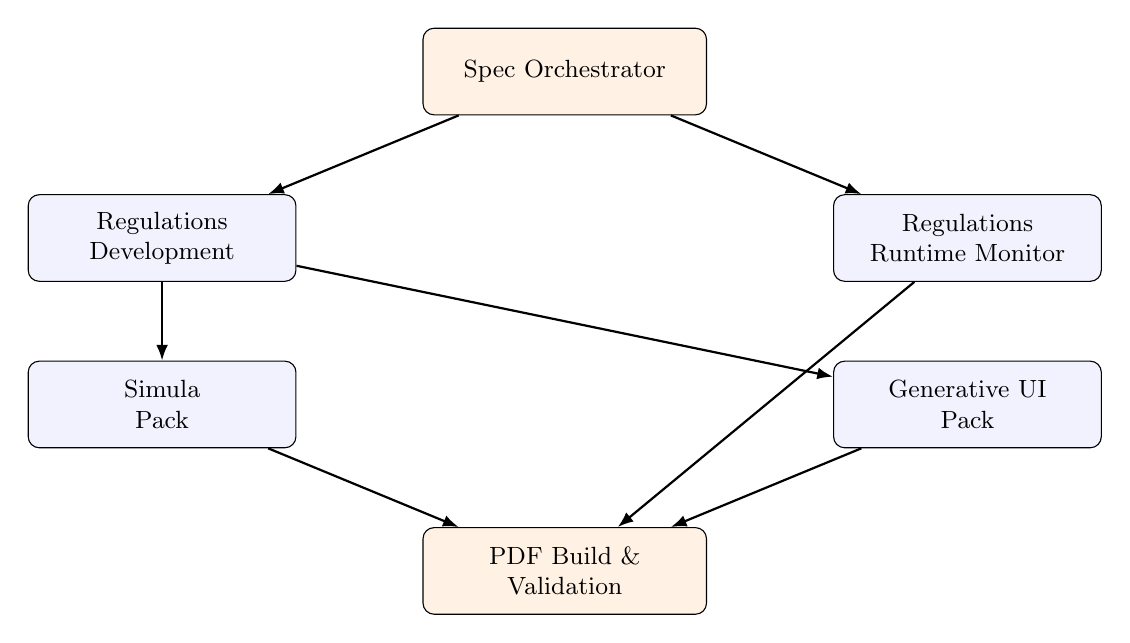
\begin{tikzpicture}[
node distance=10mm and 16mm,
box/.style={draw,rounded corners,minimum width=34mm,minimum height=11mm,align=center,font=\small,fill=blue!5},
ctrl/.style={draw,rounded corners,minimum width=36mm,minimum height=11mm,align=center,font=\small,fill=orange!10},
t/.style={-{Latex[length=2mm]},thick}
]
\node[ctrl] (lead) {Spec Orchestrator};
\node[box,below left=of lead] (regdev) {Regulations\\Development};
\node[box,below right=of lead] (regmon) {Regulations\\Runtime Monitor};
\node[box,below=of regdev] (sim) {Simula\\Pack};
\node[box,below=of regmon] (gui) {Generative UI\\Pack};
\node[ctrl,below right=of sim] (pdf) {PDF Build \&\\Validation};

\draw[t] (lead) -- (regdev);
\draw[t] (lead) -- (regmon);
\draw[t] (regdev) -- (sim);
\draw[t] (regdev) -- (gui);
\draw[t] (sim) -- (pdf);
\draw[t] (gui) -- (pdf);
\draw[t] (regmon) -- (pdf);
\end{tikzpicture}
\caption{Minimum swarm for governed spec delivery.}
\label{fig:swarm}
\end{figure}

\section{Inter-agent signaling}
\label{sec:inter-agent-signaling}

Agents within the swarm MUST NOT rely on direct network calls to each
other. All interaction SHALL be mediated via the repository state and
immutable artefacts. This constraint ensures auditability, reproducibility,
and prevents tight coupling between agent implementations.

\subsection{Signal types}

\begin{table}[htbp]
\centering
\footnotesize
\caption{Inter-agent signal types.}
\label{tab:signal-types}
\begin{tabularx}{\textwidth}{@{}l l X@{}}
\toprule
\textbf{Signal type} & \textbf{Mechanism} & \textbf{Purpose} \\
\midrule
Blocking & Lock file & Prevent downstream agents from proceeding. \\
State & JSON status file & Communicate current operational state. \\
Completion & Artefact presence & Signal that a phase is complete. \\
Degradation & Alert file & Notify swarm of service health issues. \\
\bottomrule
\end{tabularx}
\end{table}

\subsection{Blocking signals}

A runtime-monitor MUST create a lock file to signal that publication
or deployment should be halted:

\begin{table}[htbp]
\centering
\footnotesize
\caption{Blocking signal file conventions.}
\label{tab:blocking-signals}
\begin{tabularx}{\textwidth}{@{}l X@{}}
\toprule
\textbf{Path pattern} & \textbf{Meaning} \\
\midrule
\filepath{reports/alerts/<domain>\_DEGRADED.lock} & Domain is in degraded state; block PDF publication. \\
\filepath{reports/alerts/<domain>\_CIRCUIT\_OPEN.lock} & Circuit breaker is open; block all deployments. \\
\filepath{reports/alerts/SWARM\_HALT.lock} & Critical issue affecting entire swarm; halt all operations. \\
\bottomrule
\end{tabularx}
\end{table}

Lock files MUST contain:
\begin{verbatim}
{
"created_by": "<agent-identity>",
"created_at": "<ISO-8601-timestamp>",
"reason": "<human-readable-reason>",
"evidence_path": "<path-to-supporting-evidence>",
"ttl_minutes": <auto-expire-time-or-null>
}
\end{verbatim}

\subsection{State validation signals}

Before executing a deployment or migration, a development agent MUST
read the latest status file from the target domain:

\begin{itemize}
\item Path: \filepath{deployments/<domain>/status.json}
\item Required fields: \texttt{state}, \texttt{last\_updated},
\texttt{version}, \texttt{health\_check\_url}
\item The agent MUST NOT proceed if \texttt{state} is not
\texttt{HEALTHY} or \texttt{LEARNING}.
\end{itemize}

\subsection{Completion signals}

Completion is signaled by the presence of artefacts, not by explicit
messages:

\begin{table}[htbp]
\centering
\footnotesize
\caption{Completion signal artefacts.}
\label{tab:completion-signals}
\begin{tabularx}{\textwidth}{@{}l X@{}}
\toprule
\textbf{Artefact} & \textbf{Signals completion of} \\
\midrule
\filepath{docs/pdf/specs/<name>-spec.pdf} & PDF build for the named specification. \\
\filepath{reports/validation/<domain>-harness-pass.json} & Validation harness for the domain. \\
\filepath{deployments/<domain>/v<N>/manifest.json} & Deployment of version N for the domain. \\
\bottomrule
\end{tabularx}
\end{table}

\subsection{Signal consumption rules}

\begin{enumerate}
\item Agents MUST poll for signals at defined intervals (default: 30
seconds during active work).
\item Agents MUST NOT delete signals they did not create.
\item Signals older than their TTL SHALL be automatically reaped by
the repository CI service (e.g., GitHub Actions \texttt{reap-locks} job).
\item All signal creation and consumption MUST be logged to the audit
trail.
\end{enumerate}

\section{Swarm sequencing}

\begin{enumerate}
\item Freeze the regulatory control model first.
\item Update domain development packs so they inherit the regulatory
obligations.
\item Update runtime-monitor packs so they watch the resulting live
behaviour.
\item Only then assemble and publish the PDF specifications.
\end{enumerate}

\section{Non-negotiable swarm rules}

\begin{itemize}
\item No domain pack may weaken a regulations obligation locally.
\item No PDF may be treated as current if the underlying rule packs
and validation harnesses disagree.
\item Runtime-monitor agents must be able to contradict a successful
build if the live system still violates the regulations contract.
\end{itemize}
\chapter{Validation and Acceptance}
\label{ch:validation}

\section{Rule-pack validation}

Every rule-pack pair must be backed by an executable validation harness.
The harness must prove at least:
\begin{itemize}
\item the files exist at the intended paths;
\item required sections are present;
\item referenced source files and schema files exist;
\item threshold values and condition codes are explicit;
\item the pair benchmarks at least as strongly as the established
operational baseline.
\end{itemize}

\section{Recommended benchmark baseline}

The current repository baseline for operational specificity is the
Generative UI deployment rule pack at
\filepath{src/generativeUI/.clinerules}. Any new domain pack should be
benchmarked against that file for:
\begin{itemize}
\item incident memory;
\item concrete verification steps;
\item threshold explicitness;
\item checklist quality;
\item operational specificity.
\end{itemize}

\section{Quantified benchmark scorecard}
\label{sec:benchmark-scorecard}

To enable objective, reproducible comparison against the baseline, the
validation harness SHOULD compute a numeric score based on the following
metrics. This scorecard allows new domain packs to self-assess whether
they meet the ``at least as strong'' requirement.

\subsection{Scorecard metrics}

\begin{table}[htbp]
\centering
\footnotesize
\caption{Operational specificity scorecard.}
\label{tab:scorecard}
\begin{tabularx}{\textwidth}{@{}L{4.5cm} l X@{}}
\toprule
\textbf{Metric} & \textbf{Pass threshold} & \textbf{Calculation method} \\
\midrule
Explicit numeric thresholds & 100\% & All monitoring rules must specify numeric values (e.g., ``> 5\%''), not vague terms (e.g., ``high rate''). \\
Verification path density & $\ge 5$ paths per 100 lines & Count of explicit file paths referenced divided by rule pack line count, normalized to 100 lines. \emph{Note: Shorter files (< 60 lines) must contain at least 3 unique paths to avoid penalty.} \\
Known issue registry entries & $\ge 3$ entries & Count of documented previous incidents, workarounds, or known edge cases. \\
Checklist completeness & 100\% & All 11 development pack sections (or 9 runtime pack sections) must be present and non-empty. \\
Schema reference coverage & 100\% & All payload types mentioned must reference a schema file in \filepath{docs/schema/}. \\
Test entry point count & $\ge 2$ per pack & Count of explicit test file paths or commands referenced. \\
\bottomrule
\end{tabularx}
\end{table}

\subsection{Scoring algorithm}

The validation harness SHALL compute scores as follows:

\begin{enumerate}
\item \textbf{Parse the rule pack} into sections using header markers.
\item \textbf{Extract metrics}:
\begin{itemize}
\item Count threshold expressions matching pattern
\verb|[><=]+\s*\d+(\.\d+)?[%]?|.
\item Count file path references matching pattern
\verb|src/|, \verb|docs/|, or \verb|tests/|.
\item Count known issue entries in the ``Known Issues'' or
``Current Repo Reality'' section.
\item Count schema references matching pattern
\verb|\.schema\.(json|yaml)|.
\item Count test references matching pattern
\verb|test_.*\.py| or \verb|make test|.
\end{itemize}
\item \textbf{Compare against baseline}: Read the
\filepath{.baseline-clinerules-pointer} file in the repository root
to identify the current gold-standard pack (e.g.,
\filepath{src/generativeUI/.clinerules}). Load that pack and compute
the same metrics.
\item \textbf{Pass/fail determination}: A pack passes if all metrics
meet or exceed the thresholds in \cref{tab:scorecard} AND are not
worse than the baseline values.
\end{enumerate}

\section{The .baseline-clinerules-pointer}

To ensure the benchmark evolves as engineering standards mature, the
validation harness SHALL NOT hardcode the baseline pack path. This
pointer file allows the platform team to rotate the baseline without
requiring a specification update or code change to the harness.

\subsection{Scorecard output format}

The harness SHALL produce a JSON report:

\begin{verbatim}
{
"pack_path": "src/training/.clinerules",
"baseline_path": "src/generativeUI/.clinerules",
"timestamp": "2026-04-21T09:00:00Z",
"metrics": {
"threshold_explicitness": {"value": 100, "pass": true},
"path_density": {"value": 7.2, "pass": true},
"known_issues": {"value": 5, "pass": true},
"checklist_completeness": {"value": 100, "pass": true},
"schema_coverage": {"value": 100, "pass": true},
"test_entry_points": {"value": 3, "pass": true}
},
"overall_pass": true,
"baseline_comparison": "EQUAL_OR_STRONGER"
}
\end{verbatim}

\subsection{Scorecard integration}

\begin{itemize}
\item The scorecard MUST be computed as part of the CI/CD validation
gate for any PR that modifies a \filepath{.clinerules} file.
\item Scorecard results MUST be attached to the PR as a comment or
status check.
\item A pack that fails the scorecard MUST NOT be merged without
explicit exception approval (see \cref{sec:conflict-detection}).
\end{itemize}

\section{Acceptance commands}

\begin{table}[htbp]
\centering
\footnotesize
\caption{Minimum acceptance commands.}
\label{tab:acceptance}
\begin{tabularx}{\textwidth}{@{}l X@{}}
\toprule
\textbf{Area} & \textbf{Command or gate} \\
\midrule
Training rule packs & \texttt{cd src/training \&\& make test-clinerules} \\
Regulations rule packs & \texttt{cd src/intelligence/ai-core-pal \&\& make test-clinerules} \\
Regulations MCP surface & \texttt{cd src/intelligence/ai-core-pal \&\& make test} \\
Agent supplement PDF & \texttt{make spec-clinerules-agents} \\
PDF publication & \texttt{make spec-<name>} for each published book \\
\bottomrule
\end{tabularx}
\end{table}

\section{Publication criteria}

The swarm may claim a spec is delivered only when:
\begin{enumerate}
\item the relevant rule packs exist;
\item the harnesses pass;
\item the LaTeX source is committed and reference-clean;
\item the build target exists for the corresponding PDF output;
\item the runtime-monitor contract is present for any domain that is
expected to run live.
\end{enumerate}

\section{Failure conditions}

\begin{itemize}
\item Missing runtime-monitor pack for a governed live domain.
\item Rule pack cites non-existent source of truth or non-existent
verification paths.
\item Domain pack conflicts with regulations obligations.
\item PDF build succeeds but the supporting rule-pack harness fails.
\end{itemize}
\chapter{References}
\label{ch:references}

\section{Normative references}

\begin{itemize}
\item \filepath{docs/pdf/specs/regulations-spec.pdf}
\item \filepath{docs/latex/specs/regulations/chapters/03-mgf-framework.tex}
\item \filepath{docs/latex/specs/regulations/chapters/08-monitoring-spec.tex}
\item \filepath{docs/latex/specs/regulations/chapters/10-identity-attribution.tex}
\item \filepath{docs/latex/specs/regulations/chapters/12-implementation-instructions.tex}
\end{itemize}

\section{Schema references}

\begin{itemize}
\item \filepath{docs/schema/regulations/requirement.schema.json}
\item \filepath{docs/schema/regulations/conformance-tool.schema.json}
\item \filepath{docs/schema/regulations/agent-identity.schema.json}
\item \filepath{docs/schema/regulations/request-identity.schema.json}
\item \filepath{docs/schema/regulations/audit-event.schema.json}
\item \filepath{docs/schema/regulations/capability-monitoring-metrics.schema.json}
\item \filepath{docs/schema/common/exceptions-registry.schema.json}
\item \filepath{docs/schema/simula/training-example.schema.json}
\item \filepath{docs/schema/simula/taxonomy.schema.json}
\end{itemize}

\section{Repository rule-pack references}

\begin{itemize}
\item \filepath{.clinerules}
\item \filepath{src/generativeUI/.clinerules}
\item \filepath{src/generativeUI/gateway/.clinerules.runtime-monitor}
\item \filepath{src/training/.clinerules}
\item \filepath{src/training/.clinerules.runtime-monitor}
\item \filepath{src/intelligence/.clinerules}
\item \filepath{src/intelligence/.clinerules.runtime-monitor}
\item \filepath{src/intelligence/model-registry.yaml}
\item \filepath{docs/schema/common/exceptions-registry.yaml}
\item \filepath{.baseline-clinerules-pointer}
\end{itemize}

\section{Version history}
\label{sec:version-history}

\begin{table}[htbp]
\centering
\footnotesize
\caption{Document version history.}
\label{tab:version-history}
\begin{tabularx}{\textwidth}{@{}l l l X@{}}
\toprule
\textbf{Version} & \textbf{Date} & \textbf{Author} & \textbf{Changes} \\
\midrule
1.0.0 & 2026-04-15 & Platform Engineering & Initial specification release. \\
1.1.0 & 2026-04-21 & Platform Engineering & Added: rule-pack lifecycle states (\cref{sec:lifecycle-states}), baseline warm-up period (\cref{sec:baseline-warmup}), inheritance conflict detection (\cref{sec:conflict-detection}), mandatory ingress overlay (\cref{sec:ingress-overlay}), inter-agent signaling (\cref{sec:inter-agent-signaling}), quantified benchmark scorecard (\cref{sec:benchmark-scorecard}). \\
\bottomrule
\end{tabularx}
\end{table}

\section{Cross-references to other specifications}

This specification relies on and is referenced by:
\begin{itemize}
\item \textbf{Regulations Specification} (\filepath{docs/pdf/specs/regulations-spec.pdf}): Defines the governance framework that all rule packs must inherit.
\item \textbf{Simula Training Specification} (\filepath{docs/pdf/specs/simula-training-spec.pdf}): Consumes the Simula domain rule packs defined here.
\item \textbf{TB Review Specification} (\filepath{docs/pdf/specs/tb-review-spec.pdf}): May adopt the swarm delivery model for its governance needs.
\item \textbf{Arabic AP Specification} (\filepath{docs/pdf/specs/arabic-ap-spec.pdf}): May adopt the swarm delivery model for its governance needs.
\end{itemize}

\end{document}
